
\subsection{Morse and Lennard Jones Pair Potentials}

Early interatomic potentials were two-body pair potentials, where the force on an atom was determined by summing the pair potentials between that atom and other atoms in its neighbourhood, determined by a cutoff radius.

The Lennard-Jones and Morse potentials are examples of pair-potentials, but they are too simple.  They cannot capture the many-body aspect of how atoms in a metal interact with each other.  Many-body potentials such as the Finnis-Sinclair or Embedded Atom Model do have a pair potential function, and this can take the form of a LJ potential, Morse potential or other standard Pair Potentials. ... rewrite this part

\subsection{Finnis Sinclair Potentials}

Pair potentials had been used to model metals in simulations prior to EAM type potentials.  The Finnis-Sinclair potential was published in 1984 and it introduced both a pair potential and an embedded term to take into account the cohesive energy dependent on the local electron density.  The pair term represents the repulsion between the atoms whereas the embedding functional glues the atoms together in the solid.  There is no directional term, and this was ignored in the Finnis-Sinclair model; the potentials were fit as well as possible empirically.  

The embedding energy is dependent on the density function and it takes the form of a square root.



\subsection{Embedded Atom Method}


\eqEAM

Professor Howard Sheng created a website with many EAM potentials, and the plots for the three functions of the Aluminium EAM potential are shown below.

\begin{figure}[tbp]
  \begin{center}
    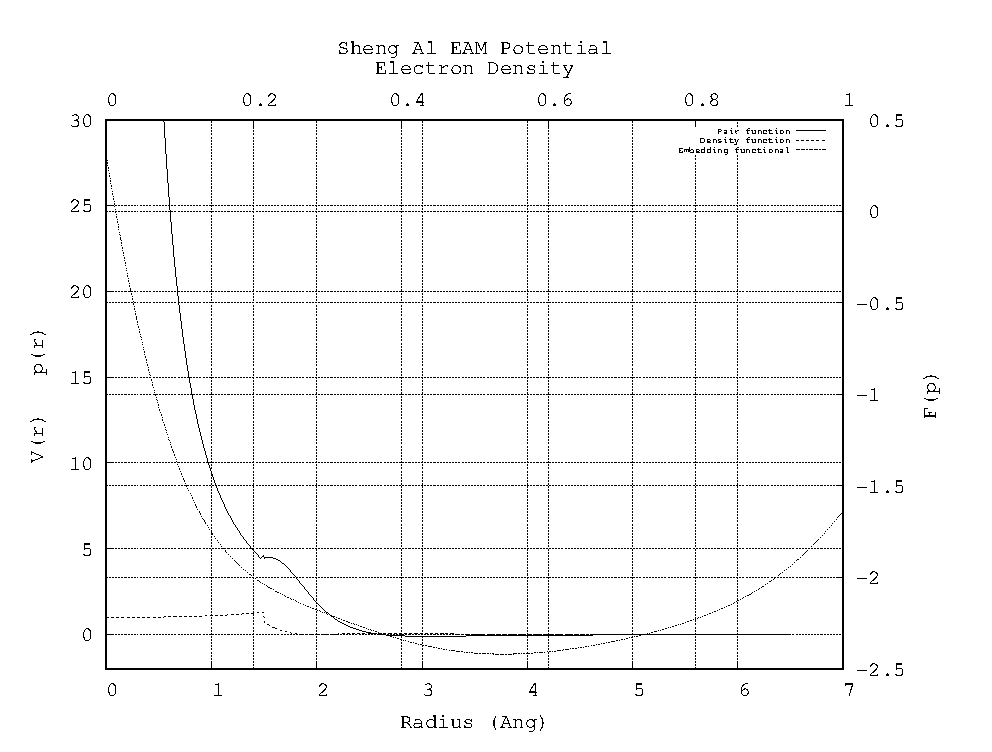
\includegraphics{chapters/background_potential_fitting/plots/sheng_eam_al}%
    \caption{Graph caption}
    \label{graph:graph1}
  \end{center}
\end{figure}

\begin{figure}[tbp]
  \begin{center}
    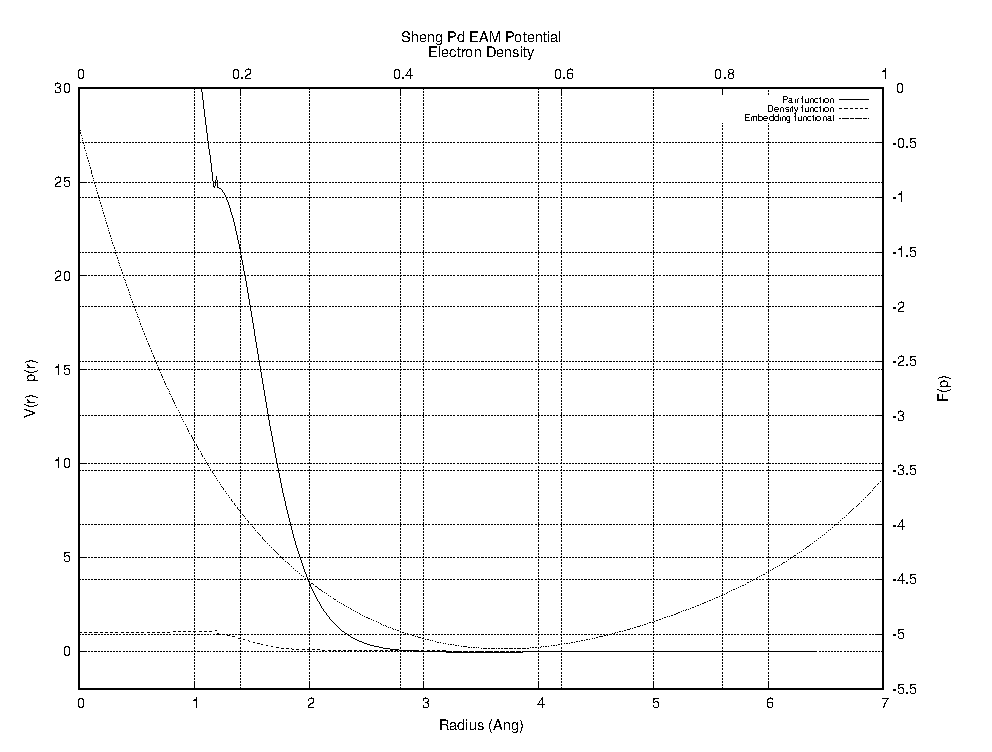
\includegraphics{chapters/background_potential_fitting/plots/sheng_eam_pd}%
    \caption{Graph caption}
    \label{graph:graph1}
  \end{center}
\end{figure}



\subsection{Two Band Embedded Atom Method}

There are several variations of the EAM potential, and one of particular interest to us is the two-band model EAM (2BMEAM) that has two electron density and embedding energy terms.  This formalism was originally developed to model Caesium (14), and the transition of electrons between S and D bands under pressure, but it has been modified to apply to alloys.

An alloy version of the two-band model was developed by Olsson et al. to investigate the α-prime phase formation in Fe-Cr (15).  It was further developed by Bonny et al to provide a reliable EAM type potential to model high-chromium ferritic alloys (16).  This potential correctly predicts the change of sign in mixing enthalpy as the local concentration of Chromium changes, and the functions take the following form.

\begin{equation}
\begin{split}
U_{EAM} = \frac{1}{2} \sum \limits_{i=1}^{N} \sum \limits_{j\ne i}^{N} V_{ij}(r_{ij}) + \sum \limits_{i=1}^{N} F_{D}[\rho _{d,i}] + \sum \limits_{i=1}^{N} F_{S}[\rho _{s,i}] \\
\textnormal{where   } \rho_{d,i} = \sum \limits_{j=i,j \ne i}^{N} \rho_{d,ij}(r_{ij})
\textnormal{  and  } \rho_{s,i} = \sum \limits_{j=i,j \ne i}^{N} \rho_{s,ij}(r_{ij})
\end{split}
\end{equation}

This allows a second embedding functional and electron density function to add/subtract energy to an atom when mixed as an alloy, but reverts to the original EAM for that element when in local concentrations of like-atoms.




